% Seccion de resultados. Numeros de tablas/numeros.tex (generados); los citados por objeto vienen de
% tablas/resultados.tex: revisarlos si se re-evalua.
\begin{table*}[!t]
\centering
\caption{Per-object results without ICP. R = real capture, T = digital twin, $\Delta$ = R $-$ T. CD: Chamfer
distance; Acc./Comp.: median accuracy/completeness; F@$\tau$: F-score at $\tau$~mm; H95: 95th-percentile
Hausdorff distance. Bold: best method for that object, domain and metric.}
\label{tab:resultados}
\resizebox{\textwidth}{!}{\scriptsize\begin{tabular}{llrrrrrrrrrrrrrrrr}
\toprule
& & \multicolumn{3}{c}{CD (mm) $\downarrow$} & \multicolumn{2}{c}{Acc. (mm) $\downarrow$} & \multicolumn{2}{c}{Comp. (mm) $\downarrow$} & \multicolumn{2}{c}{F@1 $\uparrow$} & \multicolumn{3}{c}{F@2 $\uparrow$} & \multicolumn{2}{c}{F@5 $\uparrow$} & \multicolumn{2}{c}{H95 (mm) $\downarrow$} \\
\cmidrule(lr){3-5} \cmidrule(lr){6-7} \cmidrule(lr){8-9} \cmidrule(lr){10-11} \cmidrule(lr){12-14} \cmidrule(lr){15-16} \cmidrule(lr){17-18}
Object & Method & R & T & $\Delta$ & R & T & R & T & R & T & R & T & $\Delta$ & R & T & R & T \\
\midrule
\multirow{4}{*}{Bunny-S} & NeRF & \textbf{0.87} & 0.72 & +0.15 & \textbf{0.57} & 0.51 & \textbf{0.68} & 0.59 & \textbf{0.77} & 0.86 & \textbf{0.93} & 0.97 & -0.04 & 0.99 & 0.99 & 3.1 & 2.1 \\
 & 3DGS & 0.97 & 1.32 & -0.35 & 0.71 & 0.79 & 0.82 & 0.84 & 0.65 & 0.63 & 0.92 & 0.86 & +0.06 & \textbf{0.99} & 0.96 & \textbf{2.8} & 6.7 \\
 & MVS & 1.24 & 1.30 & -0.06 & 0.75 & 0.73 & 0.99 & 0.90 & 0.56 & 0.58 & 0.84 & 0.82 & +0.02 & 0.98 & 0.97 & 4.3 & 5.6 \\
 & RGB-D & 3.07 & \textbf{0.29} & +2.78 & 2.30 & \textbf{0.14} & 3.08 & \textbf{0.33} & 0.18 & \textbf{0.98} & 0.38 & \textbf{1.00} & -0.62 & 0.86 & \textbf{1.00} & 9.8 & \textbf{0.7} \\
\midrule
\multirow{4}{*}{Bunny-L} & NeRF & \textbf{1.73} & 1.70 & +0.03 & 1.08 & 0.90 & \textbf{1.00} & 0.86 & 0.48 & 0.57 & \textbf{0.79} & 0.82 & -0.03 & \textbf{0.93} & 0.93 & 9.4 & 9.3 \\
 & 3DGS & 2.49 & 3.07 & -0.58 & 1.50 & 1.53 & 1.23 & 1.09 & 0.38 & 0.41 & 0.65 & 0.64 & +0.01 & 0.85 & 0.81 & 11.6 & 17.4 \\
 & MVS & 2.13 & 1.86 & +0.27 & \textbf{0.68} & 0.53 & 1.09 & 0.87 & \textbf{0.54} & 0.62 & 0.76 & 0.79 & -0.03 & 0.91 & 0.91 & 15.8 & 13.5 \\
 & RGB-D & 2.42 & \textbf{0.26} & +2.16 & 2.15 & \textbf{0.11} & 2.16 & \textbf{0.34} & 0.21 & \textbf{0.99} & 0.46 & \textbf{1.00} & -0.53 & 0.92 & \textbf{1.00} & \textbf{5.5} & \textbf{0.6} \\
\midrule
\multirow{4}{*}{PI2} & NeRF & \textbf{1.23} & 1.21 & +0.02 & \textbf{0.79} & 0.71 & \textbf{0.88} & 0.77 & \textbf{0.58} & 0.63 & \textbf{0.82} & 0.83 & -0.01 & \textbf{0.98} & 0.97 & 4.1 & 4.7 \\
 & 3DGS & 1.30 & 1.68 & -0.38 & 0.86 & 0.90 & 1.11 & 1.21 & 0.50 & 0.47 & 0.82 & 0.75 & +0.07 & 0.98 & 0.93 & \textbf{3.6} & 5.6 \\
 & MVS & 1.85 & 2.07 & -0.22 & 1.21 & 1.12 & 1.33 & 1.34 & 0.42 & 0.42 & 0.64 & 0.67 & -0.03 & 0.94 & 0.91 & 5.3 & 9.3 \\
 & RGB-D & 3.40 & \textbf{0.30} & +3.11 & 1.89 & \textbf{0.14} & 5.08 & \textbf{0.35} & 0.12 & \textbf{0.99} & 0.31 & \textbf{1.00} & -0.69 & 0.65 & \textbf{1.00} & 8.2 & \textbf{0.8} \\
\midrule
\multirow{4}{*}{P1} & NeRF & \textbf{1.56} & 0.83 & +0.73 & \textbf{0.90} & 0.62 & \textbf{0.80} & 0.68 & \textbf{0.56} & 0.74 & 0.77 & 0.93 & -0.17 & 0.91 & 1.00 & 7.2 & 2.4 \\
 & 3DGS & 2.24 & 1.36 & +0.87 & 1.14 & 0.99 & 1.61 & 1.11 & 0.37 & 0.47 & 0.63 & 0.83 & -0.20 & 0.87 & 0.97 & 7.5 & 4.7 \\
 & MVS & 1.59 & 1.80 & -0.21 & 1.04 & 1.04 & 1.12 & 1.22 & 0.45 & 0.45 & \textbf{0.78} & 0.70 & +0.09 & 0.95 & 0.93 & 6.2 & 6.7 \\
 & RGB-D & 1.96 & \textbf{0.27} & +1.69 & 1.51 & \textbf{0.11} & 2.27 & \textbf{0.33} & 0.26 & \textbf{0.99} & 0.52 & \textbf{1.00} & -0.48 & \textbf{0.98} & \textbf{1.00} & \textbf{4.7} & \textbf{0.8} \\
\midrule
\multirow{4}{*}{Caesar} & NeRF & \textbf{2.81} & 2.14 & +0.67 & 1.29 & 0.81 & \textbf{1.63} & 0.92 & 0.34 & 0.55 & 0.62 & 0.72 & -0.10 & \textbf{0.83} & 0.86 & 13.0 & 11.0 \\
 & 3DGS & 3.30 & 2.58 & +0.72 & 1.89 & 1.02 & 2.49 & 1.25 & 0.23 & 0.46 & 0.46 & 0.64 & -0.18 & 0.80 & 0.83 & \textbf{12.3} & 10.6 \\
 & MVS & 3.71 & 3.60 & +0.11 & \textbf{0.63} & 0.37 & 2.16 & 1.50 & \textbf{0.42} & 0.60 & \textbf{0.63} & 0.68 & -0.05 & 0.76 & 0.76 & 22.6 & 23.5 \\
 & RGB-D & 9.22 & \textbf{0.89} & +8.33 & 4.01 & \textbf{0.23} & 10.03 & \textbf{0.48} & 0.10 & \textbf{0.88} & 0.19 & \textbf{0.92} & -0.73 & 0.38 & \textbf{0.95} & 47.1 & \textbf{8.7} \\
\bottomrule
\end{tabular}
}
\end{table*}

\begin{table}[!t]
\centering\footnotesize
\caption{Mean over the \nobj\ objects. R/T: ratio of real to twin CD. ``Real + ICP'': CD after a
per-method 4-DOF ICP and mean ICP translation (mm). Time: median wall-clock per capture (RTX 2000 Ada).}
\label{tab:resumen}
\resizebox{\columnwidth}{!}{\begin{tabular}{lrrrrrrrr}
\toprule
& \multicolumn{3}{c}{CD (mm) $\downarrow$} & \multicolumn{2}{c}{F@2 $\uparrow$} & \multicolumn{2}{c}{Real + ICP} & Time \\
\cmidrule(lr){2-4} \cmidrule(lr){5-6} \cmidrule(lr){7-8}
Method & R & T & R/T & R & T & CD & shift & (min) \\
\midrule
NeRF & 1.64 & 1.32 & 1.2 & 0.79 & 0.85 & 1.62 & 0.3 & 25 \\
3DGS & 2.06 & 2.00 & 1.0 & 0.70 & 0.75 & 2.06 & 0.5 & 27 \\
MVS & 2.10 & 2.13 & 1.0 & 0.73 & 0.73 & 2.04 & 0.7 & 16 \\
RGB-D & 4.01 & 0.40 & 10.0 & 0.37 & 0.98 & 3.02 & 7.2 & 0.5 \\
\bottomrule
\end{tabular}
}
\end{table}

\subsection{Accuracy of each method in each domain}
Table~\ref{tab:resultados} lists all metrics per object, and Table~\ref{tab:resumen} their means. In the
twin, RGB-D fusion is by far the most accurate method (mean CD \rgbdS~mm, F@2~=~\rgbdFS), followed by NeRF
(\nerfS~mm), 3DGS (\gsS~mm) and MVS (\mvsS~mm). On the real captures the ranking changes: NeRF is the most
accurate (\nerfR~mm, F@2~=~\nerfFR), 3DGS (\gsR~mm) and MVS (\mvsR~mm) are tied, and RGB-D fusion becomes the
least accurate method (\rgbdR~mm, F@2~=~\rgbdFR). Fig.~\ref{fig:fscore} shows the same pattern over all
thresholds: the twin RGB-D curve saturates below 1~mm, whereas the real one reaches 0.9 only at about 10~mm.

\begin{figure}[!t]
\centering
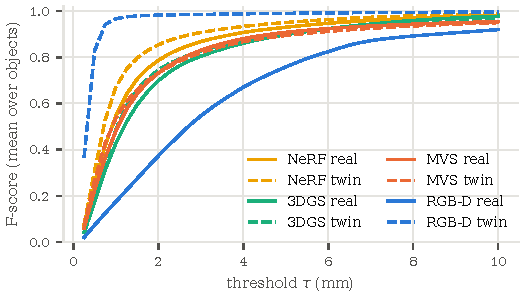
\includegraphics[width=\columnwidth]{figuras/fscore.pdf}
\caption{F-score versus threshold, averaged over the \nobj\ objects, for the real captures (solid) and their
digital twins (dashed).}
\label{fig:fscore}
\end{figure}

\subsection{Sim-to-real gap}
Fig.~\ref{fig:brecha} shows, for every object and method, the CD on the twin and on the real capture. For
the three image-based methods the twin is a good predictor of the real error: the mean gap is \nerfD~mm
for NeRF, \gsD~mm for 3DGS and \mvsD~mm for MVS (real-to-twin ratios of 1.0--1.2). Individual gaps stay
within $\pm 0.7$~mm, except for NeRF and 3DGS on the dark PETG part P1 ($+0.73$ and $+0.88$~mm) and 3DGS
on the translucent Caesar ($+0.72$~mm) (Table~\ref{tab:resultados}), where the real appearance is less favorable than the rendered one. The gap is
not always positive: 3DGS is less accurate on several twins than on the real captures (e.g., Bunny-L,
3.07 versus 2.49~mm), because its floaters depend on the rendered background and lighting, which are
approximations.

RGB-D fusion behaves differently: its mean real CD is ten times the twin value (gap \rgbdD~mm). The
per-method ICP explains most of this gap. Image-based clouds move only 0.1--1.3~mm (0.3--0.7~mm on average) when registered
individually to the CAD, i.e., they are consistent with the board frame defined by the ChArUco poses. The
RGB-D clouds move \rgbdshift~mm on average (2.5--6.4~mm for the opaque prints and 16.1~mm for Caesar), and
after this alignment the CD drops to 1.2--1.9~mm for the opaque objects, comparable to the image-based
methods. The dominant real RGB-D error is therefore a rigid offset between the L515 depth and the
photogrammetric frame, not the shape of the fused surface.

\begin{figure*}[!t]
\centering
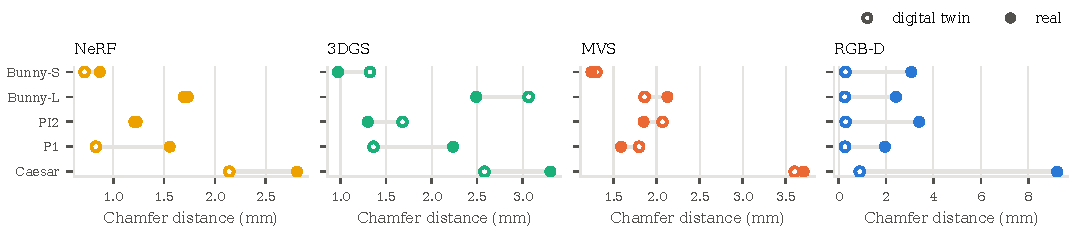
\includegraphics[width=\textwidth]{figuras/brecha.pdf}
\caption{Chamfer distance on the digital twin (hollow) and on the real capture (filled) for each object and
method. Note the different horizontal scales.}
\label{fig:brecha}
\end{figure*}

\subsection{Spatial distribution of the error}
Fig.~\ref{fig:error} shows the per-point error for the PI2 artifact. On both domains, the image-based
methods concentrate their error at concave features (the ring, the bores, the steps) and at the vertical
walls, where fewer views observe the surface; MVS additionally leaves gaps on low-texture surfaces. The
real RGB-D cloud exhibits an almost uniform error, the signature of a rigid offset, whereas its twin is
accurate everywhere.

\begin{figure*}[!t]
\centering
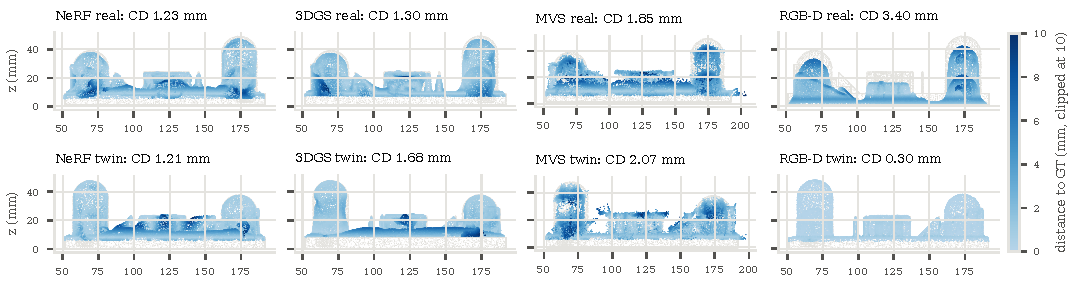
\includegraphics[width=\textwidth]{figuras/error.pdf}
\caption{Cleaned clouds of the PI2 artifact colored by distance to the CAD mesh (light gray), real capture
(top) and digital twin (bottom), side view.}
\label{fig:error}
\end{figure*}

\subsection{Effect of the material}
The translucent glow-in-the-dark PLA of Caesar is the hardest case for every method in both domains, but
especially for real RGB-D fusion: the near-infrared laser of the L515 penetrates the material, producing a
16~mm depth bias and a residual 9.0~mm CD even after ICP, an effect that the twin, which renders an opaque
material, cannot reproduce. The dark PETG of P1 increases the gap of the radiance-field methods (NeRF
$+0.73$~mm, 3DGS $+0.88$~mm) but not that of MVS ($-0.21$~mm).
